\chapter{Extension of Scalars}\label{app: extension of scalars}
For this chapter we fix a field extension $L/k$.




\section{Definition and Universal Property}


\begin{defi}
  For a $k$-vector space $V$ we define the $L$-vector spaces $V_L$ as
  \[
    V_L \coloneqq L \otimes_k V
  \]
  where the multiplication is defined as
  \[
      \lambda \cdot (l \otimes v)
    = (\lambda l) \otimes v
  \]
  for all $\lambda \in L$ and simple tensors $l \otimes v \in V_L$.
\end{defi}

To see that this multiplication is well-defined notice that for every $\lambda \in L$ the multiplication with $\lambda$ in $L$, namely
\[
          \pi_\lambda
  \colon  L
  \to     L,
  \quad   l
  \mapsto \lambda l \,,
\]
is $L$-linear and thus $k$-linear.
The multiplication with $\lambda \in L$ as defined above is simply $\pi_\lambda \otimes \id_V$.


For any $k$-vector space $V$ we have a $k$-linear inclusion
\[
                  \can_V
  \colon          V
  \hookrightarrow V_L,
  \quad           v
  \mapsto         1 \otimes v \,.
\]
The $L$-vector space $V_L$ together with the inclusion $\can_V$ satisfies an universal property.


\begin{thrm}[Universal property of the extension of scalars]
  Let $V$ be a $k$-vector space. Then for every $L$-vector space $W$ we have a natural isomorphism of $k$-vector spaces
  \begin{align*}
              \beta_W
    \colon    \Hom_L(V_L, W)
    &\to      \Hom_k(V,W) \,, \\
              f
    &\mapsto  f \circ \can_V \,,  \\
              ( \lambda \otimes v \mapsto \lambda g(v) )
    &\mapsfrom g
  \end{align*}
  This property defines $V_L$ uniquely up to unique isomorphsm:
  If $V'$ is an $L$-vector space and $\iota \colon V \to V'$ a $k$-linear map such that
  \[
            \alpha_W
    \colon  \Hom_L(V', W)
    \to     \Hom_k(V,W) \,,
    \quad   f
    \mapsto f \circ \iota
  \]
  is an isomorphism of $k$-vector spaces for every $L$-vector space $W$ then there exists an unique $L$-linear map
  \[
    \phi \colon V_L \to V'
  \]
  such that the diagram
  \begin{center}
    \tikzsetnextfilename{scalar_extension_universal_property}
    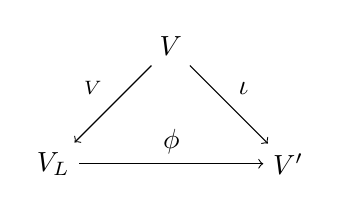
\begin{tikzpicture}[node distance = 6em, auto]
      \node (V) {$V$};
      \node (V_L) [below left of = V] {$V_L$};
      \node (V')  [below right of = V] {$V'$};
      \draw[->] (V) to node[swap] {$\can_V$} (V_L);
      \draw[->] (V) to node {$\iota$} (V');
      \draw[->] (V_L) to node {$\phi$} (V');
    \end{tikzpicture}
  \end{center}
  commutes and this map is an isomorphism of $L$-vector spaces.
\end{thrm}


That the $\beta_W$ are ``natural'' isomorphisms means the following:
Fixing a $k$-vector space $V$ we have two functors
\[
          F_1, F_2
  \colon  \cVect{L}
  \to     \cVect{k}
\]
where $F_1(W) \coloneqq \Hom_L(V_L,W)$ for every $L$-vector space $W$ and for every $L$-linear map $f \colon W \to W'$
\[
          F_1(f)
  \colon  \Hom_L(V_L, W)
  \to     \Hom_L(V_L, W'),
  \quad   h
  \mapsto f \circ h,
\]
as well as $F_2(W) \coloneqq \Hom_k(V,W)$ for every $L$-vector space $W$ and for every $L$-linear map $f \colon W \to W'$
\[
          F_2(f)
  \colon  \Hom_k(V,W)
  \to     \Hom_k(V,W'),
  \quad   h
  \mapsto f \circ h.
\]
The claim is that the $\beta_W$ form an natural isomorphism from $F_1$ to $F_2$, i.e.\ they form a natural transformation from $F_1$ to $F_2$ and $\beta_W$ is an isomorphism for every $L$-vector space $W$.


\begin{proof}
  We will start by proving that $\beta_W$ is an isomorphism of $k$-vector spaces for every $L$-vector space $W$.
  For this we fix an $L$-vector space $W$.
  It is clear that $\Phi \coloneqq \beta_W$ is well-defined and $k$-linear.
  To show that $\Phi$ is an isomorphism we show that
  \[
            \Psi
    \colon  \Hom_k(V,W)
    \to     \Hom_L(V_L, W),
            g
    \mapsto \left(
                      (\lambda \otimes v)
              \mapsto \lambda g(v)
            \right).
  \]
  is an inverse of $\Phi$.
  That $\Psi(g)$ is well-defined and $k$-linear for every map \mbox{$g \in \Hom_k(V,W)$} follows from the fact that the map
  \[
            L \times V
    \to     W,
    \quad   (\lambda, v)
    \mapsto \lambda g(v)
  \]
  is well-defined and $k$-bilinear.
  That $\Psi(g)$ is also $L$-linear is clear.
  That $\Psi$ itself is also $k$-linear is also clear.
  
  Since for all $f \in \Hom_L(V_L,W)$, $\lambda \in L$, $v \in V$
  \begin{align*}
     &\,  (\Psi \Phi)(f)(\lambda \otimes v) \\
    =&\,  \Psi(\Phi(f))(\lambda \otimes v)
    =     \Psi(f \circ \can_V)(\lambda \otimes v) \\
    =&\,  \lambda (f \circ \can_V)(v)
    =     \lambda f(\can_V(v)) \\
    =&\,  \lambda f(1 \otimes v)
    =     f (\lambda \otimes v)
  \end{align*}
  we have $\Psi \Phi = \id_{\Hom_L(V_L, W)}$ and since for all $g \in \Hom_k(V,W$, $v \in V$
  \begin{align*}
        (\Phi \Psi)(g)(v)
    &=  \Phi(\Psi(g))(v)
     =  (\Psi(g) \circ \can_V)(v) \\
    &=  \Psi(g)(\can_V(v))
     =  \Psi(g)(1 \otimes v) \\
    &=  g(v)
  \end{align*}
  we have $\Phi \Psi = \id_{\Hom_k(V,W)}$.
  
  Next we will show that the $\beta_W$ are natural isomorphisms.
  For this we need to check that for all $L$-vector spaces $W$ and $W'$ and every $L$-linear map \mbox{$f \colon W \to W'$} the diagram
  \begin{center}
    \tikzsetnextfilename{naturalisomorphism}
    \begin{tikzpicture}[node distance = 6em, auto]
      \node (HomLW) {$\Hom_L(V_L, W)$};
      \node (HomLW') [right = 6em of HomLW] {$\Hom_L(V_L, W')$};
      \node (HomkW) [below of = HomLW] {$\Hom_k(V,W)$};
      \node (HomkW') [below of = HomLW'] {$\Hom_k(V,W')$};
      \draw[->] (HomLW) to node {$F_1(f)$} (HomLW');
      \draw[->] (HomkW) to node[swap] {$F_2(f)$} (HomkW');
      \draw[->] (HomLW) to node[swap] {$\beta_W$} (HomkW);
      \draw[->] (HomLW') to node {$\beta_{W'}$} (HomkW');
    \end{tikzpicture}
  \end{center}
  commutes, where $F_1$ and $F_2$ are defined as in the previous explanation.
  This is clear, since $F_1(f)$ and $F_2(f)$ are precomposing with $f$ and $\beta_W$ and $\beta_{W'}$ are composing with $\can_V$, and therefore for all $h \in \Hom_L(V_L, W)$
  \begin{align*}
     &\,  (F_2(f) \circ \beta_W)(h)
    =     F_2(f)(\beta_W(h)) \\
    =&\,  F_2(f)(h \circ \can_V)
    =     f \circ (h \circ \can_V) \\
    =&\,  (f \circ h) \circ \can_V
    =     \beta_{W'}(f \circ h) \\
    =&\,  \beta_{W'}(F_1(f)(h))
    =     (\beta_{W'} \circ F_1(f))(h) \,.
  \end{align*}
  
  All that’s left to show is that property defines $V_L$ uniquely up to unique isomorphism.
  To prove this let $V'$ be an $L$-vector space together with a $k$-linear map $\iota \colon V \to V'$ such that for every $L$-vector space $W$ the map
  \[
            \alpha_W
    \colon  \Hom_L(V', W)
    \to     \Hom_k(V, W),
    \quad   f
    \mapsto f \circ \iota
  \]
  is an isomorphism of $k$-vector spaces.
  
  First we notice that
  \[
            \Hom_L(V_L, V_L)
    \cong   \Hom_k(V, V_L),
    \quad   f
    \mapsto f \circ \can_V.
  \]
  Therefore there exists exactly one $f \in \Hom_L(V_L, V_L)$ with $f \circ \can_V = \can_V$.
  It is clear that $f = \id_{V_L}$.
  In the same way we find that $g \in \Hom_L(V', V')$ with $g \circ \iota = \iota$ if and only if $g = \id_{V'}$.
  
  Next we notice that
  \[
            \Hom_L(V_L, V')
    \cong   \Hom_k(V, V'),
    \quad   f
    \mapsto f \circ \can_V.
  \]
  Therefore there exists a unique $L$-linear map $\phi \in \Hom_L(V_L, V')$ such that \mbox{$\iota = \phi \circ \can_V$}.
  All that’s left to check is that $\phi$ is an isomorphism.
  For this we find in same way that there exists a unique $L$-linear map $\psi \in \Hom_L(V', V_L)$ with $\can_V = \psi \circ \iota$.
  Since
  \[
      \phi \psi \circ \iota
    = \phi \circ \can_V
    = \iota
  \]
  as well as
  \[
      \psi \phi \circ \can_V
    = \psi \circ \iota
    = \can_V
  \]
  we find by the previous observations that $\phi \psi = \id_{V'}$ and $\psi \phi = \id_{V_L}$.
\end{proof}


Recall the following from linear algebra:


\begin{rec}
  Let $k$ be a field and $V$ a $k$-vector space.
  Then $B \subseteq V$ is a $k$-basis of $V$ if and only if for every $k$-vector space $W$ the restriction
  \[
        \Hom_k(V,W
    \to \Maps(B,W),
    \quad   f
    \mapsto f_{|B}
  \]
  is a bijection.
\end{rec}


\begin{lem}
  Let $V$ be a $k$-vector space.
  Then $\{v_i\}_{i \in I}$ is a $k$-basis of $V$ if and only if $\{1 \otimes v_i\}_{i \in I}$ is an $L$-basis of $V_L$.
\end{lem}
\begin{proof}
  Since $\can_V \colon V \to V_L$ is injective it induces a bijection
  \[
            \phi
    \colon  \{v_i\}_{i \in I}
    \to     \{1 \otimes v_i\}_{i \in I},
    \quad   v_i
    \mapsto 1 \otimes v_i
    =       \can_V(v_i)
  \]
  For every $L$-vector space $W$ we therefore get a commutative diagram
  \begin{center}
    \tikzsetnextfilename{scalar_extension_and_bases}
    \begin{tikzpicture}[node distance = 6em, auto]
      \node (HomL) {$\Hom_L(V_L, W)$};
      \node (Homk) [right = 6em of HomL] {$\Hom_k(V,W)$};
      \node (MapsL) [below of = HomL] {$\Maps\left( \{1 \otimes v_i\}_{i \in I}, W\right )$};
      \node (Mapsk) [below of = Homk] {$\Maps\left( \{v_i\}_{i \in I} ,W\right )$};
      \draw[double equal sign distance] (HomL) to node {$\sim$} (Homk);
      \draw[double equal sign distance] (MapsL) to node {$\sim$} (Mapsk);
      \draw[->] (HomL) to node[swap] {restriction} (MapsL);
      \draw[->] (Homk) to node {restriction} (Mapsk);
    \end{tikzpicture}
  \end{center}
  where we have an isomorphism of $k$-vector spaces
  \[
            \Hom_L(V_L, W)
    \cong   \Hom_k(V, W),
    \quad   h
    \mapsto h \circ \can_V \,,
  \]
  and the bijection
  \[
          \Maps\left( \{1 \otimes v_i\}_{i \in I}, W \right)
    \cong \Maps\left( \{v_i\}_{i \in I} ,W \right),
    \quad   h
    \mapsto h \circ \phi \,.
  \]
  That $\{v_i\}_{i \in I}$ is a $k$-basis of $V$ is equivalent to saying that the restriction on the right side is a bijection and that $\{1 \otimes v_i\}_{i \in I}$ is an $L$-basis of $V_L$ is equivalent to saying that the restriction on the left side is a bijection.
  Since the diagram commutes these two are equivalent.
\end{proof}


\begin{cor}\label{cor: inclusion to bijection vector spaces}
  Let $V$ be an $L$-vector space, $U \subseteq V$ a $k$-vector subspace and $B \subseteq U$, such that $B$ is a $k$-basis of $U$ and an $L$-basis of $V$.
  Then
  \[
            \phi
    \colon  U_L
    \colon  V,
    \quad   \lambda \otimes u
    \mapsto \lambda u
  \]
  is an isomorphism of $L$-vector spaces.
\end{cor}
\begin{proof}
  $\phi$ is the $L$-linear map that corresponds to the $k$-linear inclusion $U \hookrightarrow V$.
  Therefore it maps the $L$-basis $\{1 \otimes b\}_{b \in B}$ of $U_L$ bijectively to the $L$-basis $B$ of $V$.
\end{proof}


\begin{lem}
  Let $V$ be a $k$-vector space and $\{U_i\}_{i \in I}$ a collection of $k$-vector subspaces $U_i \subseteq V$.
  Then
  \[
      L \otimes_k \bigcap_{i \in I} U_i
    = \bigcap_{i \in I} L \otimes_k U_i \,.
  \]
\end{lem}
\begin{proof}
  {[A proof will be added later.]}
\end{proof}





\section{Functoriality}


Given $k$-vector spaces $V$ and $W$ and a $k$-linear map $f \colon V \to W$ we get a $k$-linear map
\[
            f_L
  \coloneqq \id_L \otimes f
  \colon    V_L
  \to       W_L.
\]
It is easy to check that $f_L$ is also $L$-linear.
Therefore we can understand the extension of scalars as a functor
\[
  E \colon \cVect{k} \to \cVect{L}
\]
with $E(V) = V_L$ for every $k$-vector space $V$ and $E(f) = f_L$ for every $k$-linear map $f$. 

\begin{lem}
  Let $V$ and $V'$ be $k$-vector spaces.
  For every $k$-linear map $f \colon V \to V'$
  \tikzsetnextfilename{can_and_fL_commute}
  \begin{center}
    \begin{tikzpicture}[node distance = 6em, auto]
      \node (V) {$V$};
      \node (V') [right of = V] {$V'$};
      \node (VL) [below of = V] {$V_L$};
      \node (V'L) [below of = V'] {$V'_L$};
      \draw[->] (V) to node {$f$} (V');
      \draw[->] (VL) to node {$f_L$} (V'L);
      \draw[->] (V) to node[swap] {$\can_V$} (VL);
      \draw[->] (V') to node {$\can_{V'}$} (V'L);
    \end{tikzpicture}
  \end{center}
  commutes.
\end{lem}
\begin{proof}
  This can easily be checked by calculation, since for all $v \in V$
  \begin{align*}
        (f_L \circ \can_V)(v)
    &=  f_L(\can_V(v))
     =  f_L(1 \otimes v) \\
    &=  1 \otimes f(v)
     =  \can_{V'}(f(v))
     =  (\can_{V'} \circ f)(v) \,.
    \qedhere
  \end{align*}
\end{proof}


We also have the restriction of scalars as a functor
\[
  R \colon \cVect{L} \to \cVect{k}
\]
which sends every $L$-vector space to its underlying $k$-vector space and every $L$-linear map to the corresponding $k$-linear map.
  
From the universal property of the extension of scalars we know that for every $k$-vector space $V$ and $L$-vector space $W$ we have an isomorphism
\[
          \Phi_{V,W}
  \colon  \Hom_L(E(V),W)
  \cong   \Hom_k(V,R(W))
\]
of $k$-vector spaces.
This observation results in the following proposition:
  
\begin{prop}
  $E$ is left adjoint to $R$ via the bijections $\Phi_{V,W}$.
\end{prop}
\begin{proof}
  We need to check that for all $k$-vector spaces $V$ and $V'$, all $L$-vector spaces $W$ and $W'$, every $k$-linear map $f \colon V' \to V$ (notice that $f$ goes from $V'$ to $V$) and every $L$-linear map $g \colon W \to W'$ the diagram
  \tikzsetnextfilename{scalar_extension_and_restriction_adjoint}
  \begin{center}
    \begin{tikzpicture}[node distance = 6em, auto]
      \node (L) {$\Hom_L(V_L, W)$};
      \node (L') [right = 6em of L] {$\Hom_L(V'_L, W')$};
      \node (k) [below of = L] {$\Hom_k(V,W)$};
      \node (k') [below of = L'] {$\Hom_k(V', W')$};
      \draw[->] (L) to node {$g \circ - \circ f_L$} (L');
      \draw[->] (k) to node[swap] {$g \circ - \circ f$} (k');
      \draw[->] (L) to node[swap] {$\Phi_{V,W}$} (k);
      \draw[->] (L') to node {$\Phi_{V',W'}$} (k');
    \end{tikzpicture}
  \end{center}
  commutes.
  Since $\Phi_{V,W} = - \circ \can_V$ and $\Phi_{V,W'} = - \circ \can_{V'}$ this follows from $\can_{V'} \circ f_L = f \circ \can_V$.
\end{proof}





\section{Extension of Scalars for Algebras}


Given $k$-algebras $A_1$ and $A_2$ their tensor product $A_1 \otimes_k A_2$ is a $k$-algebra via the multiplication
\[
    (a_1 \otimes b_1) \cdot (a_2 \otimes b_2)
  = (a_1 a_2) \otimes (b_1 b_2).
\]
If $A_1$ and $A_2$ are unitial, then so is $A_1 \otimes_k A_2$.
To see that this multiplication is well-defined notice that the map
\begin{align*}
            A_1 \times A_2 \times A_1 \times A_2
  &\to      A_1 \otimes_k A_2 \,, \\
            (a_1, b_1, a_2, b_2)
  &\mapsto  (a_1 a_2) \otimes (b_1 b_2)
\end{align*}
is well-defined and $k$-multilinear, so we get a $k$-linear map
\begin{align*}
            A_1 \otimes_k A_2 \otimes_k A_1 \otimes_k A_2
  &\to      A_1 \otimes_k A_2 \,, \\
            a_1 \otimes b_1 \otimes a_2 \otimes b_2
  &\mapsto  (a_1 a_2) \otimes (b_1 b_2) \,,
\end{align*}
which under the isomorphism of $k$-vector spaces
\[
        A_1 \otimes_k A_2 \otimes_k A_1 \otimes_k A_2
  \cong (A_1 \otimes_k A_2) \otimes_k (A_1 \otimes_k A_2)
\]
corresponds to a $k$-bilinear map
\begin{align*}
            (A_1 \otimes_k A_2) \times (A_1 \otimes_k A_2)
  &\to      A_1 \otimes_k A_2 \,, \\
            (a_1 \otimes b_1, a_2 \otimes b_2)
  &\mapsto  (a_1 a_2) \otimes (b_1 b_2) \,.
\end{align*}


Given a $k$-algebra $A$ we get that $A_L$ is an $L$-vector space and a $k$-algebra.
It is easy to see that that these structures are compatible and give $A_L$ the structure of an $L$-algebra.
To see this compatibility simply notice that the $k$-bilinear map
\begin{align*}
            (A_1 \otimes_k A_2) \times (A_1 \otimes_k A_2)
  &\to      A_1 \otimes_k A_2 \,, \\
            (a_1 \otimes b_1, a_2 \otimes b_2)
  &\mapsto  (a_1 a_2) \otimes (b_1 b_2) \,.
\end{align*}
is also $L$-bilinear.


\begin{rem}
  Let $A$ be a $k$-algebra.
  \begin{enumerate}[label=\emph{\alph*)},leftmargin=*]
    \item
    If $A$ is unital then so is $A_L$.
    \item
    The canonical inclusion $\can_A \colon A \to A_L$ is a homomorphism of $k$-algebras.
  \end{enumerate}
\end{rem}


\begin{lem}
  For $k$-algebras $A_1$ and $A_2$ and a homomorphism of $k$-algebras
  \[
    f \colon A_1 \to A_2
  \]
  the corresponding $L$-linear map
  \[
            f_L
    \colon  L \otimes_k A_1
    \to     L \otimes_k A_2
  \]
  is a homomorphism of $L$-algebras.
\end{lem}
\begin{proof}
  $f_L$ is multiplicative on the simple tensors since for all simple tensors $\lambda_1 \otimes a_1, \lambda_2 \otimes a_2 \in L \otimes_k A_1$
  \begin{align*}
     &\,  f_L((\lambda_1 \otimes a_1)(\lambda_2 \otimes a_2))   \\
    =&\,  f_L((\lambda_1 \lambda_2) \otimes (a_1 a_2))
    =     (\lambda_1 \lambda_2) \otimes f(a_1 a_2) \\
    =&\,  (\lambda_1 \lambda_2) \otimes (f(a_1)f(a_2))
    =     (\lambda_1 \otimes f(a_1)) (\lambda_2 \otimes f(a_2)) \\
    =&\,  f_L(\lambda_1 \otimes a_1) f_L(\lambda_2 \otimes a_2) \,.
  \end{align*}
  Since these simple tensors generate $L \otimes_k A_1$ it follows that $f_L$ is multiplicative.
\end{proof}
  
  
This shows that we can understand the extension of scalars for $k$-algebras als a functor from $\cAlg{k}$ to $\cAlg{L}$.


\begin{lem}
  Let $A$ be a $k$-algebra, $B$ an $L$-algebra and $f \colon A \to B$ a homomorphism of $k$-algebras.
  Then the corresponding $L$-linear map $\hat{f} \colon A_L \to B$ is a homomorphism of $L$-algebras.
  \begin{proof}
  Notice that for all simple tensors $\lambda_1 \otimes a_1, \lambda_2 \otimes a_2 \in A_L$ we have
    \begin{align*}
          \hat{f}((\lambda_1 \otimes a_1)(\lambda_2 \otimes a_2))
      &=  \hat{f}((\lambda_1 \lambda_2) \otimes (a_1 a_2))
       =  \lambda_1 \lambda_2 f(a_1 a_2)    \\
      &=  \lambda_1 \lambda_2 f(a_1) f(a_2)
       =  \lambda_1 f(a_1) \lambda_2 f(a_2) \\
      &=  \hat{f}(\lambda_1 \otimes a_1) \hat{f}(\lambda_2 \otimes a_2) \,.
    \end{align*}
    Since the simple tensors generate $A_L$ it follows that $\hat{f}$ is multiplicative.
  \end{proof}
\end{lem}


\begin{cor}\label{cor: inclusion to bijection algebras}
  Let $B$ be an $L$-algebra, $A \subseteq B$ a $k$-subalgebra and $X \subseteq A$, such that $X$ is a $k$-basis of $A$ and an $L$-basis of $B$.
  Then
  \[
            \phi
    \colon  A_L
    \to     B \,,
    \quad   \lambda \otimes a
    \mapsto \lambda a
  \]
  is an isomorphism of $L$-algebras.
\end{cor}
\begin{proof}
  We know that $\phi$ is a homomorphism of $L$-algebras and we have already seen that $\phi$ is an isomorphism of $L$-vector spaces.
\end{proof}


\begin{lem}
  Let $A$ be a $k$-algebra and $I \subseteq A$ a left-ideal.
  Then $I_L$ is an left-ideal in the $L$-algebra $A_L$.
\end{lem}
\begin{proof}
  Since $I$ is a $k$-vector subspace of $A$ we know that $I_L$ is an $L$-vector subspace of $A_L$.
  For $x \in A_L$ and $y \in I_L$ we have
  \[
    x = \sum_{i=1}^n \lambda_i \otimes a_i
  \]
  with $\lambda_i \in L$ and $a_i \in A$ and
  \[
    y = \sum_{j=1}^m \lambda'_j \otimes a'_j
  \]
  with $\lambda'_j \in L$ and $a'_j \in I$, and therefore
  \begin{align*}
        xy
    &=  \left( \sum_{i=1}^n \lambda_i \otimes a_i \right)
        \left( \sum_{j=1}^m \lambda'_j \otimes a'_j \right) \\
    &=  \sum_{i=1}^n \sum_{j=1}^m (\lambda_i \lambda'_j) \otimes (a_i a'_j)
    \in I_L
  \end{align*}
  This shows that $I_L$ is a left ideal in $A_L$.
\end{proof}


\begin{lem}
  Let $A$ be a $k$-algebra and $I \subseteq A$ a left-sided $k$-ideal generated by elements $(b_j)_{j \in J}$.
  Then the left-sided $L$-ideal $I_L \subseteq A_L$ is generated by the elements $(1 \otimes b_j)_{j \in J}$.
\end{lem}
\begin{proof}
  Let $I_0$ be the left-sided ideal in $A_L$ generated by the elements $(1 \otimes b_j)_{j \in J}$.
  Since $I_L$ is a left-ideal with $1 \otimes b_j \in I_L$ for all $j \in J$ we have $I_0 \subseteq I_L$.
  To show that $I_L \subseteq I_0$ we look at
  \[
              I'
    \coloneqq \{
                a \in A
              \mid
                1 \otimes a \in I_0
              \}
    =         \can_A^{-1}(I_0) \,.
  \]
  $I'$ is a left-sided ideal in $A$ since $\can_A$ is a homomorphism of $k$-algebras.
  Since $1 \otimes b_j \in I_0$ für alle $j \in J$ we have $b_j \in I'$ für alle $j \in J$.
  Since $I$ is the left ideal generated by $(b_j)_{j \in J}$ we have $I \subseteq I'$.
  Therefore we have $1 \otimes a \in I_0$ für alle $a \in I$.
  Since these simple tensors generate $I_L$ as an $L$-vector space we have $I_L \subseteq I_0$.
\end{proof}


\begin{rem}
  We have similar statements about right-sided and two-sided ideals.
\end{rem}


\begin{warn}
  The ideal $(X^2+1)_{\R[X]} \subseteq \R[X]$ is a prime ideal, but the ideal \mbox{$(X^2+1)_{\Complex[X]} \subseteq \Complex[X]$} is not.
\end{warn}





\section{Polynomial Rings and Matrix Rings}


For the polynomial ring $k[X_1, \dotsc, X_n]$ we have an $L$-algebra
\[
    k[X_1, \dotsc, X_n]_L
  = L \otimes_k k[X_1, \dotsc, X_n] \,.
\]
The interesting thing about this algebra is that is it actually $L[X_1, \dotsc, X_n]$.


\begin{prop}
  We have an isomorphism of $L$-algebras
  \[
            \Phi
    \colon  k[X_1, \dotsc, X_n]_L
    \to     L[X_1, \dotsc, X_n]0\,,
    \quad   \lambda \otimes f
    \mapsto \lambda f \,.
  \]
\end{prop}
\begin{proof}
  The monomial $X^\alpha$ with $\alpha \in \N^n$ are a $k$-basis of $k[X_1, \dotsc, X_n]$ and an $L$-basis of $L[X_1, \dotsc, X_n]$ so it follows from corollary \ref{cor: inclusion to bijection algebras}.
\end{proof}


Another interesting example of the extension of scalars is $L \otimes_k \Mat_n(k)$.


\begin{prop}
  We have an isomorphism of $L$-algebras
  \[
    \Phi \colon L \otimes_k \Mat_n(k) \to \Mat_n(L) \,.
  \]
\end{prop}
\begin{proof}
  The matrices $(E_{ij})_{1 \leq i,j \leq n}$ are a $k$-basis of $k[X_1, \dotsc, X_n]$ and an $L$-basis of $L[X_1, \dotsc, X_n]$ so it follows from corollary \ref{cor: inclusion to bijection algebras}.
\end{proof}




